
\de{ĐỀ THI ÔN TẬP  HỌC KỲ II NĂM HỌC 2022-2023}{THPT Nguyễn Thượng Hiền 10TH1}

\begin{bt}%[0D7B3-2]%HieuPhan%THPT Nguyễn Thượng Hiền 10TH1
    Giải phương trình $ \sqrt{3x^2-5x-1}=x-1 $
    \loigiai{
        Ta có \allowdisplaybreaks
       \begin{eqnarray*}
            \sqrt{3x^2-5x-1}=x-1 &\Rightarrow& 3x^2-5x-1=x^2-2x+1\\
            &\Leftrightarrow& 2x^2-3x-2=0 \Leftrightarrow \hoac{& x=2 \\ & x=-\dfrac{1}{2}.}
       \end{eqnarray*}
   Thay lần lượt $ x=2 $ và $ x=-\dfrac{1}{2} $ vào phương trình đã cho ta thấy $ x=2 $ là nghiệm của phương trình.
    }
    \end{bt}
\begin{bt}%[0D7K2-1]%HieuPhan%THPT Nguyễn Thượng Hiền 10TH1
    Tìm $ m  $ để $ f(x)=x^2-2mx+m^2-m $ luôn dương với mọi $ x $ thuộc $ \mathbb{R} $.
    \loigiai{
    $ f(x)=x^2-2mx+m^2-m $ luôn dương với mọi $ x $ thuộc $ \mathbb{R} $ khi và chỉ khi
    $$ \Delta' <0 \Leftrightarrow m^2-(m^2-m)<0\Leftrightarrow m<0. $$
    Vậy $ m<0 $ thì $ f(x)=x^2-2mx+m^2-m $ luôn dương với mọi $ x $ thuộc $ \mathbb{R} $.
}
\end{bt}
\begin{bt}%[0D8K3-2]%HieuPhan%THPT Nguyễn Thượng Hiền 10TH1
    Tìm hệ số chứa $ x^4 $ trong khai triển $ (2x-1)^5 $.
    \loigiai
    {
      Ta có 
     \begin{eqnarray*}
          (2x-1)^5 &=&\mathrm{C}_5^0(2x)^5-\mathrm{C}_5^1(2x)^4+\mathrm{C}_5^2(2x)^3-\mathrm{C}_5^3(2x)^2+\mathrm{C}_5^4(2x)-\mathrm{C}_5^5\\
          &=& 32x^5-80x^4+80x^3-40x^2+10x-1.
     \end{eqnarray*}
 Dựa vào khai triển suy ra hệ số chứa $ x^4 $ là $ -80 $.
    }
\end{bt}
\begin{bt}%[0D8Y2-1]%HieuPhan%THPT Nguyễn Thượng Hiền 10TH1
    Tổ $ 1 $ có $ 12 $ học sinh trong đó có $ 4 $ học sinh nam và $ 8 $ học sinh nữ. Có bao nhiêu cách chọn $ 3 $ học sinh làm lớp trưởng, lớp phó và thủ quỹ. (Mỗi bạn chỉ làm $ 1 $ nhiệm vụ)
    \loigiai
    {
        Mỗi cách chọn $ 3 $ học sinh từ $ 12 $ học sinh xếp vào các vị trí lớp trưởng, lớp phó và thủ quỹ là một chỉnh hợp chập $ 3 $ của $ 12 $ phần tử.\\
        Suy ra có $ \mathrm{A}_{12}^3=1320 $ cách chọn.
    }
\end{bt}
\begin{bt}%[0D0K2-2]%HieuPhan%THPT Nguyễn Thượng Hiền 10TH1
    Trong hộp có $ 3 $ viên bi xanh và $ 5 $ viên bi đỏ. Lấy ngẫu nhiên trong hộp $ 3 $ viên bi. Tính xác suất của biến cố: \lq\lq Lấy ra được $ 3 $ viên bi màu đỏ \rq\rq.
    \loigiai
    {
        Ta có $ n(\Omega) =\mathrm{C}_8^3=56$.\\
        Gọi A là biến cố ''Lấy ra được $ 3 $ viên bi màu đỏ''.\\
        Khi đó $ n(A)=\mathrm{C}_5^3=10 $.\\
        Vậy $ P(A)=\dfrac{n(A)}{n(\Omega)}=\dfrac{10}{56}=\dfrac{5}{28} $.
    }
\end{bt}

%==============Câu 6
\begin{bt}%[0H9B1-1]%Nguyễn Mộng Hùng%THPT Nguyễn Thượng Hiền 10TH1
	Trong mặt phẳng $Oxy$ cho $A(5;3)$, $B(3;7)$, $C(-2;-8)$. Tìm tọa độ điểm $D$ sao cho $ABCD$ là hình bình hành.
\loigiai{
	Gọi $D(x;y)$. Khi đó $\overrightarrow{AD}=(x-5;y-3)$, $\overrightarrow{BC}=(-5;-15)$.\\
	Tứ giác $ABCD$ là hình bình hành, suy ra\\
	$$\overrightarrow{AD}=\overrightarrow{BC}\Leftrightarrow\heva{&x-5=-5\\&y-3=-15}\Leftrightarrow\heva{&x=0\\&y=-12.}$$
	Vậy $D(0;-12)$.

}
\end{bt}
%==============Câu 7
\begin{bt}%[0H9B2-2]%Nguyễn Mộng Hùng%THPT Nguyễn Thượng Hiền 10TH1
	Cho ba điểm $A(-3;2)$, $B(3;4)$, $C(9;-2)$. Viết phương trình tổng quát và phương trình tham số của đường cao $AH$.
	\loigiai{
	Ta có $\overrightarrow{BC}=(6;-6)$, suy ra véc-tơ cùng phương với $\overrightarrow{BC}$ là $\vec{n}=(1;-1)$.\\
	Do $AH\perp BC\Rightarrow\vec{n}=(1;-1)$ là véc-tơ pháp tuyến của đường cao $AH$.\\
	Phương trình tổng quát của đường cao $AH$ là
	$$1(x+3)-1(y-2)=0\Leftrightarrow x-y+5=0.$$
	Vì $\vec{n}=(1;-1)$ là véc-tơ pháp tuyến của đường cao $AH$, suy ra $\vec{a}=(1;1)$ là véc-tơ chỉ phương của đường cao $AH$.\\
	Phương trình tham số của đường cao $AH$ là
	$$\heva{&x=-3+t\\&y=2+t}, t\in\mathbb{R}.$$
}
\end{bt}


% câu 8
\begin{bt}%[Hiếu Mai]%[0T9K3-6]
Một cái cổng hình bán nguyệt rộng $ 6{,}8 \, \text{m} $, cao $ 3{,}4 \, \text{m} $. Mặt đường dưới cổng được chia thành hai làn cho xe ra vào.
\begin{center}
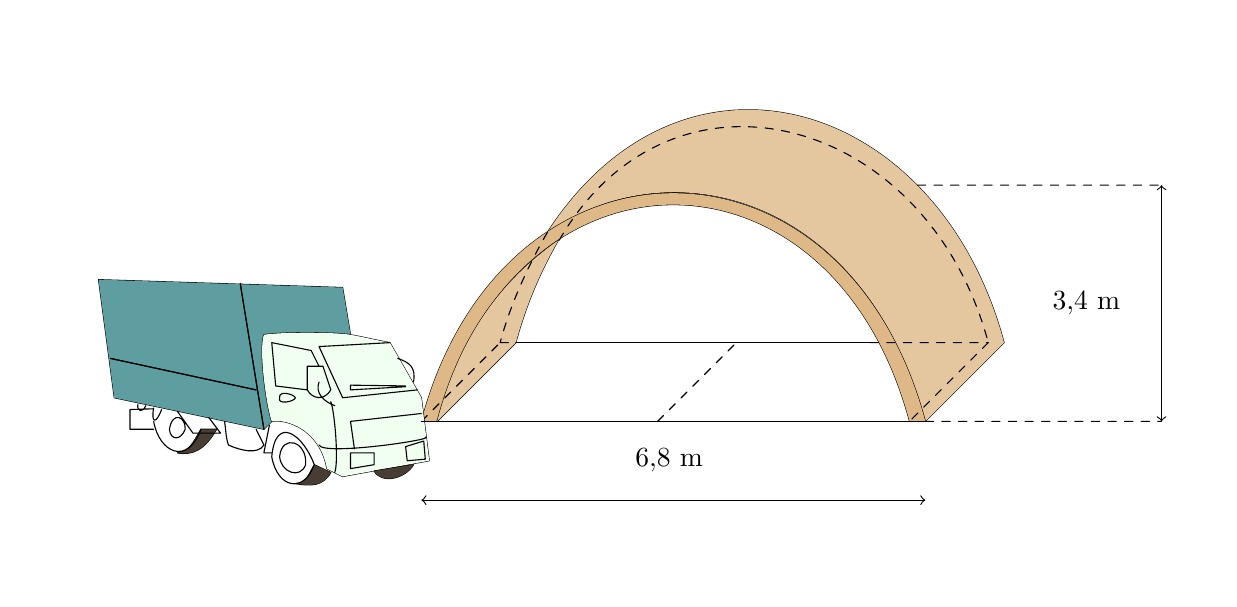
\begin{tikzpicture}[line join=round, line cap=round,scale=1,transform shape]
\definecolor{burlywood}{rgb}{0.87, 0.72, 0.53}
\definecolor{cadetblue}{rgb}{0.37, 0.62, 0.63}
\definecolor{honeydew}{rgb}{0.94, 1.0, 0.94}
\definecolor{darklava}{rgb}{0.28, 0.24, 0.2}
\clip (-8,-4) rectangle (7,3);

\tikzset{chen/.pic={

\def\C{ 
(4.4,-1)..controls +(105:3.2) and +(57:3.2) ..(-1.4,.4)
..controls +(35:1.9) and +(105:3) ..(3.4,-2)--cycle
;}
\draw\C;
\fill[burlywood!80] \C;

\def\B{  (-2.8,-2)
..controls +(75:3.8) and +(105:3.8) ..(3.2,-2)--(3.4,-2)
..controls +(105:4) and +(75:4) ..(-3,-2)--cycle;
}
\draw\B;
\fill[burlywood] \B;

\def\D{ 
(-1.26,.3)
..controls +(-120:.45) and +(75:.5) ..(-1.8,-1)--
(-2.8,-2)
..controls +(75:1) and +(-145:1) ..cycle
;}
\draw\D;
\fill[burlywood!80] \D;

\draw[dashed](-2,-1)--(-1.8,-1)
%..controls +(77:3.8) and +(105:3.8) ..(4.2,-1)--(4.4,-1)
(-1.4,.4)
..controls +(-120:.5) and +(75:.5) ..(-2,-1)
(-1.25,.3)..controls +(60:2.85) and +(105:3) ..(4.2,-1)
(4.2,-1)--(3.2,-2)
(-3,-2)--(-2,-1)
;
\def\ThanXe{ 
(-7.1,-.2)--(-4,-.3)--(-3.9,-.9)
..controls +(170:.2) and +(10:.2) ..(-5,-.9)
..controls +(-110:.2) and +(110:.2) ..(-4.9,-2)--(-5,-2.1)--(-6.9,-1.7)--cycle

;}
\draw\ThanXe;
\fill[cadetblue] \ThanXe;
\draw (-5,-2.1)--(-5.3,-.25) (-6.95,-1.2)--(-5.1,-1.6);
\def\DauXe{ 
(-3.9,-.9)
..controls +(170:.2) and +(10:.2) ..(-5,-.9)
..controls +(-110:.2) and +(110:.2) ..(-4.9,-2)
..controls +(10:.2) and +(100:.5) ..(-4.2,-2.6)--(-4,-2.7)--(-2.9,-2.5)--(-3,-1.7)--(-3.4,-1)
..controls +(170:.2) and +(-10:.2) ..cycle
;}
\draw\DauXe;
\fill[honeydew] \DauXe;
\draw (-5,-2.1)--(-5.3,-.25) (-6.95,-1.2)--(-5.1,-1.6)
(-3.4,-1)--(-4.3,-1.05)--(-4,-1.7)--(-3.05,-1.6)
(-3.9,-1.54)--(-3.2,-1.55)--(-3.2,-1.56)--(-3.9,-1.6)--cycle
(-4.9,-1)--(-4.4,-1.1)--(-4.3,-1.3)--(-4.45,-1.3)--(-4.45,-1.6)--(-4.85,-1.55)--cycle
(-4.3,-1.3)--(-4.45,-1.3)--(-4.45,-1.6)
..controls +(-60:.15) and +(-120:.15) ..(-4.15,-1.6)--(-4.25,-1.3)--cycle
(-4.3,-1.5)
..controls +(-110:.15) and +(160:.15) ..(-4.1,-1.8)
(-4.15,-1.75)
..controls +(-70:.15) and +(70:.15) ..(-4.1,-2.65)
(-4.3,-2.3)
..controls +(-70:.15) and +(-10:.15) ..(-2.95,-2.2)
(-3.85,-2.35)--(-3.9,-2)--(-3,-1.9)
(-3.9,-2.6)--(-3.9,-2.4)--(-3.6,-2.4)--(-3.6,-2.55)--cycle
(-3.18,-2.5)--(-3.2,-2.32)--(-2.97,-2.25)--(-2.95,-2.48)--cycle
;
\def\BanhXe{ 
(-3.6,-2.63)
..controls +(-60:.2) and +(-120:.2) ..(-3.1,-2.55)--cycle

(-4.36,-2.55)--(-4.15,-2.65)
..controls +(-120:.2) and +(-10:.2) ..(-4.6,-2.79)
..controls +(5:.15) and +(-120:.2) ..cycle
%-------------------
(-5.8,-2.1)--(-5.6,-2.1)
..controls +(-120:.3) and +(-10:.2) ..(-6.1,-2.4)
..controls +(5:.15) and +(-120:.2) ..cycle
;}
\draw\BanhXe;
\fill[darklava] \BanhXe;
\draw (-4.9,-2.45)
..controls +(-80:.4) and +(-110:.4) ..(-4.36,-2.55)
(-4.9,-2.45)
..controls +(85:.55) and +(110:.4) ..(-4.36,-2.55)
(-4.8,-2.45)
..controls +(-85:.2) and +(-110:.2) ..(-4.47,-2.55)
(-4.8,-2.45)
..controls +(85:.3) and +(85:.3) ..(-4.47,-2.55)
(-6.2,-2.1)
..controls +(-85:.15) and +(-110:.15) ..(-6,-2.1)
(-6.2,-2.1)
..controls +(80:.25) and +(85:.15) ..(-6,-2.1)
(-4.9,-2.4)--(-5,-2.4)--(-4.93,-2.05)
(-5.1,-2.1)--(-5,-2.3)
..controls +(-120:.15) and +(-25:.15) ..(-5.45,-2.3)
..controls +(110:.1) and +(-80:.1) ..(-5.5,-2)
(-5.7,-1.95)--(-5.55,-2.15)--(-5.9,-2.15)--(-6.1,-1.87)
(-6.3,-1.85)
..controls +(-110:.2) and +(-100:.2) ..(-6.4,-1.83)
(-6.5,-1.8)
..controls +(-110:.1) and +(-100:.1) ..(-6.6,-1.78)
(-6.4,-2.1)--(-6.7,-2.1)--(-6.7,-1.85)--(-6.4,-1.84)
(-4.8,-1.7)
..controls +(-110:.1) and +(-100:.05) ..(-4.6,-1.7)
..controls +(110:.05) and +(100:.1) ..cycle
(-3.3,-1.2)
..controls +(-20:.15) and +(80:.2) ..(-3.1,-1.5)
%-----------
(-6.4,-2)
..controls +(-80:.4) and +(-110:.5) ..(-5.8,-2.1)
;
}}

\path
(0,0)pic[scale=1]{chen};
\draw (-1.8,-1)--(2.7,-1) (-3,-2)--(3.4,-2);
\draw[dashed] (2.7,-1)--(4.2,-1)
(3.4,-2)--(6.4,-2) (3.3,1)--(6.4,1) (0,-2)--(1,-1);
\draw[<->] (6.4,-2)--(6.4,1);
\draw[<->] (-3,-3)--(3.4,-3);
\node at (6,-.5) [left]{$3{,}4$ m};
\node at (.7,-2.5) [left]{$6{,}8$ m};
\end{tikzpicture}
\end{center}

\begin{enumerate}
	\item Viết phương trình mô phỏng cái cổng.
	\item Một chiếc xe tải rộng $ 2{,}4 \, \text{m} $ và cao $ 2{,}5 \, \text{m} $ đi đúng làn đường quy định có thể đi qua cổng được hay không?
\end{enumerate}
\loigiai{
\begin{center}
\begin{tikzpicture}[>=stealth, scale=1.4, declare function={r=3.4; w=2.4; h=2.5;}]
	\draw[->] (-5,0) -- (5,0) node[above] {$ x $};
	\draw[->] (0,-1) -- (0,5) node[right] {$ y $};
	\draw[very thick, brown] (r,0) arc [start angle=0, end angle=180,radius=r];
	\node at (60:r+1) {$ (C) \colon x^2 + y^2 = r^2 $};
	\draw[dashed, <->] (0,0) -- (135:r) node[pos=.5, sloped, above] {$ r=3{,}4\,\text{m} $};
	\draw[very thick, red] (0,0) rectangle (w,h);
	\foreach \x/\y/\n/\a in {0/0/O/-135, w/0/A/-90, 0/h/C/180}{
		\fill[black] (\x,\y) circle (1.5pt) + (\a:.3) node {$ \n $};
	}
	\fill[black] (2.4,2.5) circle (1.5pt) node[anchor=south west] {$ B(2{,}4;2{,}5) $};
\end{tikzpicture}
\begin{enumerate}
	\item Viết phương trình mô phỏng cái cổng.
	\\
	Đặt trục của cổng đi qua tâm $ (O) $ và vuông góc với mặt phẳng $ (Oxy) $ của hệ trục tọa độ $ Oxy $ như hình vẽ. Cái cổng có bán kính $ r = 3{,}4 \, \text{m} $ nên phương trình của nửa đường tròn mô tả cổng là
	$$
		(C) \colon x^2+y^2 = 1\,156 \quad (y \ge 0)
	$$
	\item Một chiếc xe tải rộng $ 2{,}4 \, \text{m} $ và cao $ 2{,}5 \, \text{m} $ đi đúng làn đường quy định có thể đi qua cổng được hay không?
	\\
	Xe tải được mô phỏng bằng hình chữ nhật $ OABC $.
	Xe có thể đi qua hay không ta cần xét xem điểm $ B(2{,}4;2{,}5) $ nằm trong hay ngoài nửa đường tròn $ (C) $. Ta thấy
	$$
		OB = \sqrt{(2{,}4)^2+(2{,}5)^2} = 3{,}5 > r \quad (3{,}5 > 3{,}4)
	$$
	nên điểm $ B $ nằm ngoài nửa đường tròn $ (C) $. Do vậy xe tải không thể đi qua cổng.
\end{enumerate}
\end{center}
}
\end{bt}

% câu 9
\begin{bt}%[Hiếu Mai]%[0T9K4-0]%THPT Nguyễn Thượng Hiền 10TH1
Một vệ tinh chuyển động quanh Trái Đất theo một quỹ đạo là một elip mà Trái Đất là một tiêu điểm.
Elip có chiều dài trục lớn và trục nhỏ lần lượt là $ 86\,724 \, \text{km} $ và $ 80\,606 \, \text{km} $.
Tính khoảng cách ngắn nhất và khoảng cách dài nhất từ tâm Trái Đất đến vệ tinh, biết rằng các khoảng cách đó đạt được khi Trái Đất và vệ tinh nằm trên trục lớn của elip.
\loigiai{
\begin{center}
\begin{tikzpicture}[>=stealth, scale=1.3]
	\draw[->] (-6,0) -- (6,0) node[above] {$ x $};
	\draw[->] (0,-4) -- (0,4) node[right] {$ y $};
	\draw[thick] (0,0) ellipse (5cm and 3cm);
	\draw[thick, brown] (-3,0) circle (28pt) + (90:1.3) node {Trái Đất};
	\draw[thick, red] (5,0) circle (17pt) + (45:1.1) node {vệ tinh};
	\foreach \x/\y/\n/\a in {0/0/O/-135, -3/0/F_1/-90, -5/0/A_1/135, 5/0/A_2/-45}{
		\fill[black] (\x,\y) circle (1.5pt) + (\a:.3) node {$ \n $};
	}
\end{tikzpicture}
\end{center}
Gọi $ \dfrac{x^2}{a^2} + \dfrac{y^2}{b^2} = 1 $ với $ a,b \ne 0 $ là phương trình elip mô tả quỹ đạo chuyển động của vệ tinh xung quanh Trái Đất. Theo đề bài, ta thấy
$$
	\heva{
		&2a = 86\,724 \\
		&2b = 80\,606
	}
	\Rightarrow
	\heva{
		&a = 43\,362 \\
		&b = 40\,303
	}
$$
Trái Đất ở vị trí $ F_1(-c,0) $.
Khoảng cách từ vệ tinh tới Trái Đất lớn nhất khi vệ tinh ở vị trí $ A_2(a,0) $ và nhỏ nhất khi nó ở vị trí $ A_1(-a,0) $ với
$$
	c = \sqrt{a^2-b^2} 
	= \sqrt{(43\,362)^2-(40\,303)^2}
	= 15\,998
$$
Khi đó 
$$
	\heva{
		&A_2F_1 = OF_1 + OA_2 = c + a = 15\,998 + 43\,362 = 59\,360 \\
		&A_1F_1 = OA_1 - OF_1 = a - c = 43\,362 - 15\,998 = 27\,364
	}
$$
Vậy khoảng cách từ vệ tinh tới Trái Đất lớn nhất là $ 59\,360 \, \text{km} $ và nhỏ nhất là $ 27\,364 \, \text{km} $.
}
\end{bt}
